\documentclass[10pt,a4paper,twocolumn]{article}

\usepackage[T1]{fontenc}
\usepackage[utf8]{inputenc}

\usepackage[english]{babel}
\usepackage{natbib}
\usepackage{url}

\usepackage{subfigure}

\usepackage{graphicx, grffile}
\graphicspath{{../assets/}}

\usepackage{booktabs}

\title{Personal Reflections: Some thoughts on writing}
\author{Nazarov Ivan}

\begin{document}
\maketitle

I, personally, find the following guidelines and methods useful and productive for
writing text and pouring thoughts onto digital medium. They may be naive or silly, but
it think it is worth documenting them here. By the way this text itself may not follow
them by the letter, but hopefully does not gravely violate them.

Below is a brief recollection of what urged me to compose this scribble in early
Autumn of 2019:
\begin{quote}
  I used to follow them, but then lost my way due to stress and personal issues and
  forgot what it feels to actually `Feel` these principles. Luckily, such us the human
  nature, that one Wednesday evening, feeling particularly down from the paper that
  dragged on and on, I decided to force myself into not putting fragments, but complete
  thoughts into the text. I began a new document and pushed myself into getting a hold
  of my scattered ideas about composing text, they once again dawned onto me. I seem
  to have rebounded.
\end{quote}

Anyway, below are the guidelines, that strive for one goal: writing better quality
narrative in my academic/personal texts (not that many have been written so far, though).

\section{Avoid sentence/thought fragments} % (fold)
\label{sec:avoid_sentence_thought_fragments}

As soon as possible and not later, but always coalesce fragments into complete sentences
and/or coherent text fragments.

The train of thought is orders of magnitude faster than typing. Thus it is permitted
to write sentences/text out of order, skipping ahead to compose the ending or key phrases,
and backtracking afterwards to fill in the gaps. Place the pieces where ever they seem
to be relevant or belong in the tentative plan of the text.

Try to formulate what you want to write (at least crudely and partially) before actually
writing -- some planning and thought does ignite the mind and put you in the "flow".
It is not forbidden to type and design a sentence in Russian (native language), before
actually translating it to English.

% section avoid_sentence_thought_fragments (end)

\section{Fractal text structuring} % (fold)
\label{sec:fractal_text_structuring}

The overall narrative follows the classic structure: from general to specific. We introduce
something, develop it, draw conclusions, and move on either by getting more specific, or
shifting focus onto the connected topic or related concept. Focus on a single idea within
a paragraph, section, plot, or table.

Paragraph contains one complete piece of thought and its structure is the same: intro-%
main-outro, -- with cohesive devices interspersed here and there to string them together.
Paragraphs themselves exist within this narration flow: some paragraphs introduce, other
relay ideas concepts and the rest summarize or draw conclusion from the narrative in the
former.

% section fractal_text_structuring (end)

\section{The text is malleable material} % (fold)
\label{sec:the_text_is_malleable_material}

Writing text can benefit from programming styles and techniques. Adopt modular hierarchical
treatment of sentences, paragraphs, and sections. Top-down writing style works wonders:
begin with coarse plan, then progressively refine its element and ultimately being
coalescing the letters into words into phrases, into sentences, into paragraphs and
sections.

Always try to come up with synonyms when writing sentences -- this increases variety,
and broadens the perspective.

% section the_text_is_malleable_material (end)

\section{Iterative process} % (fold)
\label{sec:iterative_process}

Writing text is an iterative process of constant addition, removal, refinement and
revision. Just like research: submit for feedback, update, then rinse and repeat.

\begin{figure}
  \centering
  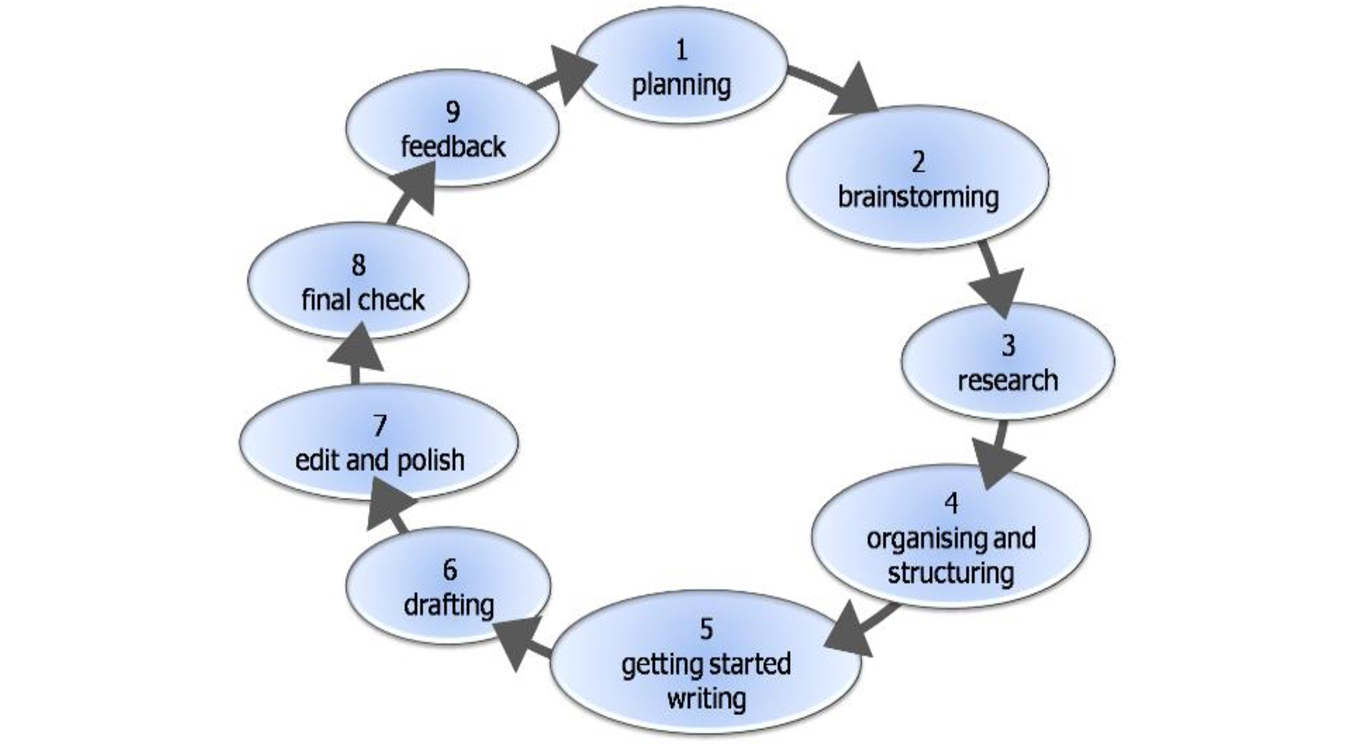
\includegraphics[width=\columnwidth]{assets/iterative_process.pdf}
  \caption{
    The cyclic process of writing.
  }
\end{figure}

% section iterative_process (end)

\section{General narrative guidelines} % (fold)
\label{sec:general_narrative_guidelines}

The following rules are mostly listed as imperatives.

Don't include things (text, sentence, ideas) that are not your point. Do not add a formula
just for the sake of a formula. The narrative must flow: introduce concepts before using
them, refer to them as necessary, or even reproduce their condensed versions when needed.
Connect and develop ideas within text: what is the focus now builds upon what came before.
Try to keep related things close to each other -- that way it requires much less cognitive
load to understand the main idea of the paragraph, section or text.

% section general_narrative_guidelines (end)

\section{Writing and research} % (fold)
\label{sec:writing_and_research}

% some general words
Research is finding answers to questions using appropriate methods (fig.~\ref{fig:direction}).
It is an process of systematic analysis of available information and prior findings
aimed at providing insight and conclusions. The process is aimed at testing carefully
formulated hypotheses and proposals using methods designed or selected with due care
and attention. Ultimately research relates to the synthesis of new actionable in broad
sense knowledge, based on the existing theory, past findings and original insight.

Research is carried out with the intent of making relevant contribution to the field. It
relies on organized and closely analysed materials, including prior art, which informs
its own direction and focus. The focus is put in the context of the current state of its
discipline: relevant theoretical basis, recurrent issues and topics, historic and current
debates, various perspectives and significant contributions.
\begin{figure}
  \centering
  \begin{subfigure}
    \centering
    \includegraphics[width=\columnwidth]{assets/direction.png}
  \end{subfigure}%
  \begin{subfigure}
    \centering
    \includegraphics[width=\columnwidth]{assets/research_context.png}
  \end{subfigure}
  \caption{
    Obvious in hindsight.
  }
  \label{fig:direction}
\end{figure}

The core part of the research is its written account, which details the process, hypotheses,
and methods, brings out significance of the findings (``so what?''), spells out implications
and conclusions. The write up demonstrates the progression of the chain of research findings
and critically evaluates the findings in context.

% lit review and context
The context of the research in the write up is contained in the literature review, related
work, and discussion sections. They help build the narrative by providing coverage and
analysis of the relevant knowledge base, significant prior research and key issues. In the
course of the narrative the context is interpolated onto the present findings, is drawn
upon for comparison, criticism, explanation or support. Context is built on broad reading,
is aware of a wide range or related work, yet remains focused on carefully curated prior
research and specialized papers, their contributions and limitations.

% As an integral part of research activity, writing is not done after everything is carried out.
Writing must be an integral part of research activity, not a step done after the experiments.
In science you start with a hypothesis, test it then toss it out -- all of this reflected
in text. Text is dispensable: each writing activity is useful, but do not cling to text,
code or any other literary expression.

Having many drafts is normal and encouraged: each draft must be checked for assumptions,
terminology, logical correctness.

A seemingly good advice is to try writing an early draft of the conclusion, which might
give a solid sense of direction, and used as a reminder of the research hypothesis. Since
the findings are written up on-the-go, this draft will inevitably be updated to reflect the
recent developments, contradictory or refuting evidence.

% getting started and managing
Like every project, research requires advanced resource management skills: work process
organization and planning, self-management, time management, scheduling, and risk assessment.

% reword this
When setting out to research a new topic, it is important to develop a sense of the method
needed to arrive at the expected answer to the posed question in the ``end product''. Having
this understanding will help make task scheduling easier and manageable.
%
Begin by diligently surveying the field, focusing reading and thinking on potential topics,
and formulate research questions and hypotheses. Then think how you will answer the question
or test the hypothesis and develop a detailed overview of the basic process, considering
potential complexities.
%
Then prepare the materials, fine-tuning thinking, research question and methods. Start project
planning process, detailing tasks and steps and making sense of what they entail. Identify and
clarify steps and work out the best order. But don't dive right in, orient yourself with the
task from start to finish. Always keep accurate and coherent records of what you do, organize
your to-do lists and logs, set writing targets.

% section writing_and_research (end)

\section{Reflections on managing} % (fold)
\label{sec:reflections_on_managing}

Key characteristics of a dissertation as a project:
\begin{itemize}
  \item scale -- substantial workload at each stage
  \item unique -- original piece of work (replication is ok)
  \item informed -- draw upon the previous research, methods, findings, and theory, relevant
  and up-to date
  \item focused on a single topic, which is covered in depth, but also put into perspective
  \item time bound -- can easily run out of time if time is not managed well
  \item well managed -- close attention to detail and excellent forward planning: start with
  thinking how to manage work overall, identify advance preparation required to ensure each
  step in completed in time
\end{itemize}

Managing the project as a process, which enables you to deliver on the set out research
goals, and relates to organization, planning, scheduling and coordination.
\begin{figure}
  \centering
  \begin{subfigure}
    \centering
    \includegraphics[width=\columnwidth]{assets/staged_process.png}
  \end{subfigure}%
  \begin{subfigure}
    \centering
    \includegraphics[width=\columnwidth]{assets/planning_before.png}
  \end{subfigure}
  \caption{
    ``Organization'' is everything.
  }
  \label{fig:organization}
\end{figure}

Key steps
\begin{enumerate}
  \item form an overview
  \item enumerate the scope and elaborate on the task
  \item plan a systematic approach to working out how you complete all component tasks
  \item manage resources, identify and manage risks (hedging)
  \item implement self- and time- management strategies
  \item formulate the ``big picture'' as clearly as possible: develop and understanding
  of the field, consider the rationale for setting such assignments and tasks
  \item elaborate the scope: clarify the outputs, level of detail, quality
  \item clarify the overall process to produce the outputs, then simplify
  \item work out the scope of tasks after having a clear mental structure
  \item detail the process, tasks and their relationships
  \item list and schedule tasks in the process
\end{enumerate}

Plan each step closely in order to minimize unwanted surprises and delays Leave some
slack, be flexible at the start of the project to ensure feasible plans
\begin{itemize}
  \item be ready to consider the whole process in detail more than once, pondering about
  how it fits together
  \item fine-tune the plans as the result of reading and research
  \item be prepared to rethink everything in detail as the project unfolds
\end{itemize}

Planning is iterative the more you discover and get to know, the more rich planning picture will become

Forward planning for concurrent and out-of-sequence tasks
\begin{itemize}
  \item identify tasks you need to address only once
  \item carefully consider tasks that are recurrent (optimization, scheduling)
\end{itemize}

% if you ever get to superwise your own students, ask them to perform a literature search
% and analysis like in the porject on Intellectual Property:
% * analysis of relevance, key ideas and results
% * juxtaposition against prior research, criticism
% * write up of the literature search findings
Develop a system (devices) that suits you and helps you with scheduling, planning and to
take stock of the progress.
\begin{enumerate}
  \item fig.~\ref{fig:organization}
  \item literature search, surveying, brainstorming followed by checking feasibility
  and methodology
  \item clarify exactly what are you setting out to investigate: write hypotheses, devise
  research plan, strategy or method
  \item focus on reading the materials, keeping notes details: write up a review, synthesize
  what has been achieved and its significance of your research
  \item implement the research design: fine-tune and write up the methods, collect data
  and analyze
  \item collate data, summarize results and their significance
  \item Discuss findings, draw conclusions and bring critical analysis to the methods
  (scope, limitations), identify directions for further research, discuss implications and
  recommendations
  \item outline the report, rework the drafts, making sure that
  \begin{itemize}
    \item arguments and details are consistent and come across clearly from beginning to end
    \item the narrative is coherent, structured, clear and cognitively easy to follow
    \item to rewrite anything that sounds muddled, to make less wordy and more succinct
    \item to check if earlier sections need rewriting or updating
  \end{itemize}
\end{enumerate}

% Unforeseen challenges and eventualities
consider what realistically can go wrong and how to deal with such eventualities.
Immediately ask for clarification.

Perfectionism: constantly reworking the assignments, considering it unworthy to submit.
Be realistic about when the proposal is good enough, adhere to detailed scheduling.

Being swept away by enthusiasm, rather than working out carefully what is practicable.
Failure to understand the implications for not finding material or collecting data.
Not having looked into the topic sufficiently before deciding on the proposal.

% self-management
At times levels of enthusiasm and interest dip, exacerbated by
\begin{itemize}
  \item lack of structure, apparent complexity (planning, engagement)
  \item high level of autonomy (not feeling up to the task)
\end{itemize}
Things to be prepared for:
\begin{itemize}
  \item difficulty of getting down to work
  \item waning interest in the research
  \item hard to motivate to undertake tasks the need doing
  \item failing to see where the research is heading
  \item having to put effort just into managing myself to keep going
\end{itemize}

Keep in mind the benefits of what you're doing: become an expert, develop research and 
project management skills.

Nurture intellectual curiosity
\begin{itemize}
  \item stimulate your intellect: fresh inspiration and wider perspectives benefit work
  \item read more broadly, even outside of my area, take inquisitive approach (what if?
  so what?)
  \item browse the origins, look for more than one way of resolving a question
\end{itemize}

% expertise
\begin{itemize}
  \item tap in your existing expertise
  \item anchoring yourself by going back over your previous work, skills and knowledge
\end{itemize}

% Confidence
\begin{itemize}
  \item encountering something problematic or challenging is not the same as being bad at it
  \item expert $=$ time $\cdot \bigl($reading $+$ thought$\bigr)$
  \item No self pity or deprecation. Just do. ``do better, do differently, or don't''
  \item think forward: how might I follow up with further research, given the opportunity
\end{itemize}

% Risks
\begin{itemize}
  \item new publications in my field that mean changing my methods and interpretations
\end{itemize}

% Incentives
\begin{itemize}
  \item if one big incentive ceases to inspire, come up with a new reason
  \item schedule rewards after completed work
\end{itemize}
\begin{figure}
  \centering
  \includegraphics[width=\columnwidth]{assets/plan_task_reward.png}
\end{figure}

% on time
Time is the most valuable resource
\begin{itemize}
  \item underestimating how long things take to do
  \item not bringing an assignment or task to an end
  \item not settling down to study or work, losing momentum, finding it hard to keep going
\end{itemize}

List tasks to do across the lifetime of the project, apart from the project itself:
unforeseen emergencies, family, leisure, job. Use planning tools to map out all demands
on time
\begin{itemize}
  \item regular times in the day to check the planner
  \item sort out time conflicts as soon as they emerge
  \item jot down a list of specific tasks to complete in a given time, this provides
  tasks as soon as you sit down to work
\end{itemize}
Break the task into more manageable units, and chip away at the larger tasks bit by bit.
Front-loading -- do more than you think is necessary early on. Contingencies -- put in
extra 10\% time, overcompensate in your planning, rather than taking the risk of running
out of time.
% If you are bored at the early stages of the project, consider changing it, while there still is time.

% Bringing an assignment to an end
settle for good enough: excessive perfectionism is a barrier to completion. The nature
of writing and research is such that there will always be something extra to add, new
related work to summarize, a better way to write up a piece of text.

Maintaining momentum: 
\begin{itemize}
  \item jump start: ``once you complete one task, spend a few minutes thinking or storming
  ideas on the next task on the list''. Read through the plan to check what to do next,
  or jot down some ideas for it
  \item avoid dwelling in the lost or wasted time: focus on the time left
\end{itemize}

% On supervisor
It is not reasonable to expect the supervisor
\begin{itemize}
  \item to find things out for me, rather than pointing me in the right direction
  \item be a particular kind of person, or my friend: although they should make
  sure to provide a constructive and friendly working environment
\end{itemize}

% section reflections_on_managing (end)

% Working with the problem pitch: Examine the brief
The brief is the formal set of requirements that you need to meet to pass the assignment.
\begin{itemize}
  \item read the brief at least twice, summarizing it in my own words
  \item What is the purpose? What parameters are fixed, and what is up to me to decide? Can
  I choose the research hypotheses? What and due when are the interim and final deliverable
  outputs? What are the standards and criteria?
\end{itemize}

% choosing a topic
Picking the topic and methodology
\begin{itemize}
  \item motivated: imagination, genuine interest, worthwhile problem, relevant to
  career, identity, or life interests
  \item challenging: sufficiently complex to feel stretched intellectually, adding to
  my prior knowledge and skills
  \item grounded: related to a subject I am familiar with and have a fairly good grasp
  of (in terms of theories, methodologies, lore)
  \item feasible: not over-ambitious (scale down the focus), immense or too complex,
  reasonably completable within the allotted time, not to exquisite for there to be
  second to no related established work or research
  \item original and contributory: the topic not studies by anyone else in exactly the
  same manner with the same kind of interpretations: materials, data, methodology, conclusions
\end{itemize}
Have a clear rationale for studying the proposed topic, be clear about the methods.
Synthesize ideas from multiple varied sources. Pick a manageable topic, avoid topics
with scant research base.

Sources for ideas of a topic:
\begin{itemize}
  \item journal and book reviews, paper criticisms, gaps or limitations in methodology
  or theory
  \item recurrent themes within the field or adjacent research where similar hypotheses
  are tested, but under slightly varying conditions
\end{itemize}

Enumerating topics:
\begin{enumerate}
  \item cover as broadly as possible the potential sources of ideas and maintain a list
  \item narrow down the range, settle on a single broad area of interest
  \item broaden and specialize the chosen area
  \item eliminate topics that are complicated or time-consuming to research
\end{enumerate}

Developing the idea:
\begin{itemize}
  \item reading widely: read exactly on the topic, read related subjects in order to
  generate ideas and become aware of other perspectives
  \item free association: jot down everything that comes to mind when reflecting on
  the topic
\end{itemize}

% Grice's Maxims of making a title, written text and conversation
The title of the proposal; must be clear, specific, incorporating a question and an
answer, precise.
\begin{itemize}
  \item The maxim of quantity: be as informative as possible, and give as much information
  as is needed, and no more
  \item The maxim of quality: be truthful, and do not give information that is false or
  not supported by evidence
  \item The maxim of relation: be relevant and pertinent to the discussion
  \item The maxim of manner: be as clear, as brief, and as orderly as possible, avoid
  obscurity and ambiguity
\end{itemize}

% doing the literature search and review
Develop breadth of understanding, gather ideas for the topic and frame the vector (context)
of research, identify the key contributions of my topic.

% general
Searching for relevant information: keywords, related terms, skimming forward and reverse
citations. Curating and analysing the collected materials: deciding what to keep or exclude.
Writing the literature review in a critically analytical way.

% staged process
Write as you go and apply critical thinking:
\begin{enumerate}
  \item reading:
  \begin{enumerate}
    \item initial browsing to scout the field
    \item detailed search of related material
    \item careful selection and vetting of what to read
    \item in-depth engagement with the key reading matter
  \end{enumerate}
  \item analysis:
  \begin{enumerate}
    \item making decisions on how to draw upon prior research (ideas, theory, methodology,
    background material)
    \item understanding the connections and influences
  \end{enumerate}
  \item use:
  \begin{enumerate}
    \item refer back to literature context when analysing data, experiments, when using
    or developing methods, when discussing the findings, when drawing the conclusions
    \item compare and contrast, synthesize, use as hypotheses, ideas, interpretation
  \end{enumerate}
\end{enumerate}

% keeping reading manageable
\begin{itemize}
  \item focus only on the related work, be ruthless while reading and pay attention only
  to relevant sections of text, keep to the point, read context, and conclusions
  \item summarize information in your own words, avoid copy-pasting text
\end{itemize}

% what to focus on?
\begin{itemize}
  \item recurrent issues, debates, gaps in research, future research directions
  \item methods and challenges in the field
  \item origins and important foundations, chain of contributions, influences
  trajectory of the field, continuations,
  \item key inventors, researchers and players, applications
\end{itemize}
Gradually as you continue reading and collecting material for the topic, the reading
must become more specialized in content and more relevant of the topic, reflective about
findings, analytical and critical of the covered material.

% refrences
a passing reference, a sentence for more significant pieces of work, several sentences
for important research, paragraphs for discussing exceptionally important research.

The purpose of literature review is
\begin{itemize}
  \item to indicate a key phase in the progress of the field
  \item draw attention to developments and limitations of theoretical base (methodology),
  critique thereof
  \item make reference to findings, to insights ad ideas drawn upon in my research
  \item illustrate the point, use as evidence in support of or contradiction to own findings
\end{itemize}

Charting and mapping for synthesis
\begin{itemize}
  \item origins (themes, ideas, motivations), direction of travel, contribution
  \item go back and forth through the context chain to keep relevant material and keep
  track of influence
  \item make a succinct summary of previous research and theory, but only of what is
  relevant and has a bearing on own project
  \item write the literature review, keeping in mind its relevance to the narrative of
  the write up: how does this enrich or build the cognitive experience of the reader? how
  is this related to the subject matter?
\end{itemize}

% on methodology
Methodology is the overarching approach to research:
\begin{itemize}
  \item the big ``how'' and ``why'' issues from which decisions about how to carry out
  the research logically follow
  \item research paradigms, i.e. broad overarching framework, integrated set of assumptions
  about how research should be conducted), the role of the researcher, theories
\end{itemize}

Approaches: empiricism, grounded theory, scientific (positivist), action.

Scientific take a neutral detached stance in pursuit of indisputable objective facts.
Goals are: testing hypotheses, establishing cause and effect, i.e. distinguishing coincidental
  co-occurrence, from causality by controlling research conditions (fig.~\ref{fig:scientific_cycle}).
\begin{figure}[t]
  \centering
  \includegraphics[width=\columnwidth]{assets/scientific_cycle.png}
  \caption{
    theory - observation - analysis cycle
  }
  \label{fig:scientific_cycle}  
\end{figure}

Historical approach: relates to particular, rather then universal truths, by asking factual,
rather than counterfactual questions, and examining rich reconstruction of the past time,
theme or event, obtained by triangulating evidence across different scattered sources,
records and accounts.

Grounded theory: takes data and inductively builds theory hypotheses on top of it

Action research: like A~/~B testing, but related to professional practice.
\begin{itemize}
  \item identify issue or problem, then work in a 4-stage cyclical process:
  plan, undertake the action, observation, and reflection
  \item researcher is an integral part of the change process, rather then an ``outsider''
\end{itemize}

% making the research proposal
There is no point in seeking approval for a proposal that you don't really believe you
can pull though, or in which you already see major flaws.

A solid proposal must
\begin{enumerate}
  \item demonstrate my solid knowledge and understanding of the topic and the field (read
  widely, examine different perspectives, jot down ideas, weigh up options, achieve clear
  thinking)
  \item summarize the prior findings as the foundation of my own research, what similar
  hypotheses have been tested?
  \item identify the topic (issue, gap, limitation), varying angles, make sure there is
  no ambiguity about the purpose of the research (avoid hesitancy or vagueness, express
  actions)
  \item articulate thesis or hypothesis (proposition and initial premise, ``condition A
  results in outcome B for reason C''): precise, clear and succinct summary of expectations,
  the core message (this is clear reference point for the project)
  \item indicate the parameters, and what precisely the research covers
  \item methodology: brief details of methods and theoretical framework, design the research
  in such a way as to test theory or hypotheses as clearly as possible, to see whether it can
  be supported by evidence.
  \item feasibility: scope and scale of the project, tentative plan and road map
  \item risks
\end{enumerate}

A hypothesis can either be disproven or provided supporting evidence (a specific set of
conditions). A hypothesis can structure the write up:
\begin{enumerate}
  \item results: state whether the research findings supported the research hypothesis or not
  \item discussion: examine the reasons that gave rise to the findings, and why the hypotheses
  were or were not supported by evidence
  \item abstract: state the hypotheses, whether the results support them, at what level
  of significance, and what is the contribution
\end{enumerate}

the pilot
\begin{itemize}
  \item a succinct, critical outline of what worked, any flaws that became aparent, what
  would improve and fine-tune the research
  \item describe what you set out to do, what has been done, and what is the outcome
\end{itemize}

\end{document}
